\documentclass[11pt,a4paper]{article}

% TACL Template Style
% Use [hyperref,submission] for anonymous review submissions
% Use [hyperref,acceptedWithA] for camera-ready / internal archival versions with author names displayed
\usepackage[hyperref,submission]{tacl2021v1}

% Standard package imports
\usepackage{times}
\usepackage{latexsym}
\usepackage{amsmath}
\usepackage{amssymb}
\usepackage{graphicx}
\usepackage{booktabs}
\usepackage{multirow}
\usepackage{microtype}
\usepackage{url}
\usepackage{xcolor}
\usepackage{array}

% Set graphics search paths
\graphicspath{{figures/final/}{figures/}{figures/source/}}

\title{Cross-Lingual Evidence Verification: Verifier Prediction Sensitivity Under Hindi-to-English Translation Shift}

% Author metadata (Visible when [acceptedWithA] option is passed to tacl2021v1; obscured under [submission])
\author{Onkar Kharat\textsuperscript{1} \quad Himanshu Jadhav\textsuperscript{2} \\
  \textsuperscript{1}Lead Researcher, Cross-Lingual Evidence Verification Project \\
  \textsuperscript{2}Co-Author \& Research Contributor \\
  \texttt{Repository: https://github.com/Onkar-Kharat/research-crosslingual-rag} \\
}

\date{}

\begin{document}
\maketitle

\begin{abstract}
Cross-lingual claim verification systems frequently convert non-English evidence texts into intermediate English representations prior to automated veracity classification. However, translating evidence introduces a critical tension between exploiting high-capacity English language models and introducing semantic distortion. In this study, we present a controlled empirical investigation of verifier prediction sensitivity under Hindi-to-English translation shift on authentic claim-evidence pairs from the X-Fact benchmark ($N=266$: 103 development, 163 held-out test). Holding the claim, pre-retrieved evidence snippets, and cross-lingual verifier (\texttt{mDeBERTa-v3-base}) fixed, we evaluate veracity decisions across four paired conditions: \emph{No-Check} (machine-translated English evidence), \emph{Direct Multilingual} (original Hindi evidence), \emph{Always-Check} (unconditional posterior consensus), and a risk-calibrated \emph{Selective-Check} cascade tuned on development data ($\tau^*=0.650$).

We observe an overall paired prediction disagreement rate of 63.80\% (104/163; 95\% CI: [56.19\%, 70.78\%]) between original and translated evidence representations. When translated evidence predicts \textsc{Supported}, evaluating the original Hindi evidence flips the prediction to \textsc{Contradicted} in 48.44\% of cases (31/64). Direct Multilingual verification achieves 42.94\% accuracy (70/163), significantly outperforming the No-Check baseline (28.22\%, 46/163; McNemar exact $p = 0.008772$, $b=27, c=51$). However, risk-calibrated Selective-Check does not surpass No-Check accuracy (28.22\%, 46/163; coverage 7.98\%), and paired permutation tests on class-balanced Macro-F1 reveal no statistically significant difference across conditions ($p = 0.1898$ and $p = 0.1180$), reflecting the high variance of harmonic metrics under severe natural class skew (87.12\% \textsc{Contradicted}, 0.0\% gold \textsc{Supported}). We transparently document the exploratory nature of this evaluation, the prior inspection of the test split, and the necessity of pending bilingual human validation before causal translation claims can be substantiated.
\end{abstract}

\section{Introduction}
\label{sec:intro}

Automated claim verification and fact-checking are essential technical defenses against misinformation across multilingual digital ecosystems \citep{thorne-etal-2018-fever,gupta-srikumar-2021-xfact}. In retrieval-augmented generation (RAG) and evidence-grounded verification architectures operating in multilingual environments, retrieved evidence passages frequently originate in a language different from the claim or the primary training language of the downstream verifier \citep{lewis-etal-2020-rag,liu-etal-2025-xrag}.

To address multilingual discrepancies, practical verification architectures routinely adopt a ``translate-then-verify'' paradigm: source-language evidence snippets are machine-translated into English bridge sequences before being processed by a cross-lingual entailment model \citep{ranaldi-etal-2026-multilingual,singhal-etal-2024-comparative}. While projecting into an English bridge format allows systems to leverage high-capacity English language models, machine translation can subtly distort fine-grained factual relationships, including named entities, negation scope, numerals, and temporal qualifiers \citep{singhal-etal-2024-comparative}. Conversely, cross-lingual verifiers evaluating original evidence directly (\emph{Direct Multilingual}) avoid translation artifacts but may exhibit reduced reasoning accuracy in lower-resource languages or incur substantial latency penalties \citep{wang-etal-2026-languages,conneau-etal-2020-unsupervised}.

While recent literature has actively examined cross-lingual RAG for generative question answering \citep{liu-etal-2025-xrag,ranaldi-etal-2026-multilingual} and uncovered language bias in dense document rerankers \citep{wang-etal-2026-languages}, previous studies have largely treated evidence translation as a monolithic utility. As a result, two fundamental empirical questions remain unresolved for cross-lingual claim verification:
\begin{enumerate}
    \item \textbf{Prediction Sensitivity Under Translation Shift:} When an identical claim and evidence passage are evaluated by the same cross-lingual verifier, to what extent do predictions flip between the original language and machine-translated representations, and what specific directional transitions characterize this disagreement?
    \item \textbf{Efficacy of Selective Original-Evidence Fallback:} Can a lightweight, test-time risk trigger (combining verifier predictive uncertainty and numeral overlap) selectively consult original evidence, and does such a selective cascade improve overall veracity accuracy compared to translated-only and unconditional dual-language consensus?
\end{enumerate}

To address these questions, we establish a controlled empirical investigation using authentic journalistic fact-checks from the Hindi partition of the X-Fact benchmark \citep{gupta-srikumar-2021-xfact}. By holding the claim, retrieved evidence snippets, verifier architecture (\texttt{mDeBERTa-v3-base}; \citealt{he-etal-2021-deberta,laurer-etal-2024-less}), and decoding configuration fixed across paired conditions, we isolate the specific sensitivity of the verifier to evidence language representation.

We define four paired conditions:
\begin{itemize}
    \item \textbf{No-Check (Translated English Only):} Evaluates machine-translated evidence passages ($e_{\text{trans}}$).
    \item \textbf{Direct Multilingual (Original Hindi Only):} Evaluates original Hindi evidence passages ($e_{\text{orig}}$).
    \item \textbf{Always-Check (Dual Consensus):} Unconditionally averages class posterior distributions from both representations.
    \item \textbf{Selective-Check:} Employs a risk-gated cascade tuned strictly on development data ($\tau^*=0.650$), consulting original Hindi evidence only when predictive uncertainty or numeral mismatch is elevated.
\end{itemize}

\paragraph{Scope and Empirical Guardrails.}
To ensure strict research integrity, we explicitly define the boundaries of this study:
\begin{itemize}
    \item \emph{Evidence Representation, Not End-to-End RAG:} This study evaluates pre-retrieved evidence snippets; upstream retrieval mechanisms and downstream generative answer synthesis are not varied.
    \item \emph{Observational Model Sensitivity, Not Translation Causality:} Without completed bilingual human validation, model prediction disagreement cannot be definitively attributed to translation distortion. All findings are reported as observational prediction sensitivity.
    \item \emph{Exploratory Diagnostic Evaluation:} Because the test split ($N=163$) was evaluated during earlier exploratory research, all evaluations are designated as diagnostic rather than confirmatory holdout testing.
    \item \emph{Dataset Imbalance Disclosure:} The official X-Fact Hindi test partition contains 142 \textsc{Contradicted} and 21 \textsc{Insufficient\_Evidence} instances, and exactly zero gold \textsc{Supported} instances. Accuracy and nominal Macro-F1 are analyzed as secondary descriptive proxies rather than general fact-checking capabilities.
\end{itemize}

\paragraph{Key Findings.}
Our empirical results on the test partition reveal:
\begin{enumerate}
    \item \textbf{Substantial Prediction Disagreement:} Verifier predictions disagree across language representations on 63.80\% of instances (104/163; 95\% CI: [56.19\%, 70.78\%]).
    \item \textbf{Pronounced Directional Flips:} When translated evidence predicts \textsc{Supported}, evaluating the original Hindi evidence flips the prediction to \textsc{Contradicted} on 48.44\% of cases (31/64).
    \item \textbf{Accuracy Disparity and McNemar Significance:} Direct Multilingual achieves 42.94\% accuracy (70/163), significantly outperforming the No-Check baseline (28.22\%, 46/163; McNemar exact $p = 0.008772$, $b=27, c=51$).
    \item \textbf{Selective Cascade Limitations:} Selective-Check ($\tau^*=0.650$) triggers on 7.98\% of test instances (saving 59.2\% compute relative to Direct Multilingual) but matches No-Check accuracy exactly (46 vs. 46, 28.22\%; McNemar exact $p = 1.0000$). On development data, the zero-check baseline utility ($J=0.2104$) exceeds the cascade peak ($J=0.2023$).
    \item \textbf{Metric Discordance Under Class Skew:} While accuracy gains for Direct Multilingual are statistically significant under McNemar's paired test, paired permutation tests on class-balanced Macro-F1 ($B=5,000$, seed 42) do not reach significance ($p=0.1898$ and $p=0.1180$), demonstrating the vulnerability of harmonic metrics under severe benchmark class imbalance.
\end{enumerate}

\section{Related Work}
\label{sec:related_work}

We situate our empirical investigation at the intersection of multilingual retrieval-augmented generation, cross-lingual claim verification, translation distortion in downstream NLP, and selective classification cascades.

\subsection{Multilingual and Cross-Lingual RAG}
Retrieval-augmented generation (RAG) grounds language model predictions in external non-parametric evidence passages \citep{lewis-etal-2020-rag}. In multilingual settings, systems must bridge linguistic gaps when queries, evidence documents, or downstream generation targets diverge in language. \citet{liu-etal-2025-xrag} formalize cross-lingual RAG (XRAG) across diverse language pairs (e.g., Arabic, Chinese, German, Spanish, English), demonstrating that retrieving evidence across languages introduces severe generative drift and syntactic interference during answer synthesis. To mitigate multilingual knowledge disparities, \citet{ranaldi-etal-2026-multilingual} introduce CrossRAG, which converts non-English search contexts into an intermediate English representation prior to generative decoding by an English reader model. While CrossRAG demonstrates empirical gains on open-domain question answering benchmarks (MKQA, MLQA, XOR-TyDi), it evaluates continuous text generation where downstream decoders can tolerate mild paraphrase variance. In contrast, claim verification requires sharp, discrete entailment decisions where subtle semantic shifts induce categorical veracity flips.

Concurrently, investigations into cross-lingual indexing bias demonstrate that neural retrieval and reranking systems systematically prioritize English-centric documents over non-English counterparts \citep{wang-etal-2026-languages,conneau-etal-2020-unsupervised}. While \citet{wang-etal-2026-languages} examine upstream retrieval representation bias, our work investigates the complementary downstream stage: holding pre-retrieved evidence fixed, how sensitive is the veracity decision of a multilingual verifier to evidence language representation?

\subsection{Cross-Lingual Fact and Claim Verification}
Automated fact verification has expanded from monolingual English benchmarks such as FEVER \citep{thorne-etal-2018-fever} to multi-language and real-world claim contexts. The X-Fact benchmark \citep{gupta-srikumar-2021-xfact} introduced naturally occurring fact-checks across 25 languages, reflecting authentic journalistic claims labeled by professional fact-checkers. Recent comprehensive benchmarking on X-Fact by \citet{shcharbakova-etal-2025-scale} reveals a critical architectural insight: fine-grained claim verification on low- and medium-resource languages remains an immense challenge for large generative language models (7B--12B parameters), which frequently succumb to multilingual hallucination, whereas specialized multilingual encoder-based NLI verifiers (\texttt{mDeBERTa-v3}, \texttt{XLM-RoBERTa}) consistently achieve superior evidence grounding and calibration \citep{he-etal-2021-deberta,laurer-etal-2024-less}. However, \citet{shcharbakova-etal-2025-scale} evaluate evidence passages strictly in their scraped source language, leaving the interaction between machine translation and multilingual verification unexamined.

\subsection{Translation Shift and Semantic Distortion}
The ``translate-then-verify'' paradigm rests on the assumption that translation bridges language barriers without perturbing factual content. However, machine translation systems \citep{tiedemann-thottingal-2020-opus} frequently suffer from subtle hallucinations, mistranslation of named entities, altered numerical quantities, and dropped negation markers. In an exploratory evaluation of multilingual fact-checking with LLMs, \citet{singhal-etal-2024-comparative} observed that pipeline translation into English frequently deteriorated classification accuracy in low-resource languages. Nevertheless, prior literature has treated translation degradation as a monolithic aggregate drop, failing to provide directional transition analyses, paired statistical hypothesis tests, or diagnostic error stratifications.

\subsection{Selective Prediction and Cascade Verification}
Selective prediction (or classification with a reject option) enables models to abstain or defer uncertain predictions to a more capable or expensive oracle \citep{geifman-elyaniv-2017-selective}. In cost-sensitive NLP, cascade architectures route easy queries to lightweight, low-latency models and difficult queries to large models. We adapt this principle to cross-lingual verification: rather than unconditionally translating or unconditionally running heavy dual-language models, we evaluate whether a lightweight risk gating mechanism can selectively trigger original-language verification only when the translation path exhibits high predictive uncertainty or surface-level entity corruption.

\subsection{Summary of Literature Positioning}
Table~\ref{tab:prior_work_matrix} summarizes how this study relates to and differs from prior work across task, language setting, architecture, evaluation design, and empirical focus. Our study does not claim to present a new foundation model or a universally optimal RAG pipeline. Instead, it provides the first rigorously controlled, paired empirical characterization of verifier prediction sensitivity under Hindi-to-English translation shift, establishing transparent directional transition matrices and identifying the fundamental diagnostic challenges posed by benchmark class imbalance.

\begin{table*}[t]
\centering
\small
\resizebox{\textwidth}{!}{
\begin{tabular}{p{3.2cm}p{2.8cm}p{2.8cm}p{3.2cm}p{2.8cm}p{4.2cm}}
\toprule
\textbf{Study} & \textbf{Task} & \textbf{Language Setting} & \textbf{Method / Architecture} & \textbf{Evaluation} & \textbf{Key Distinction from Present Study} \\
\midrule
\citet{liu-etal-2025-xrag} & Open-domain generative QA & Multilingual (ar, zh, de, es, en) & Generative LLM with cross-lingual dense retrieval & QA Exact Match, language drift & Evaluates continuous text generation; does not study discrete 3-way claim verification or prediction transitions. \\
\addlinespace
\citet{ranaldi-etal-2026-multilingual} & Knowledge-intensive QA & Multilingual (MKQA, MLQA, XOR-TyDi) & CrossRAG: Translate retrieved passages to English & Span F1 / EM on QA answers & Assumes translation is universally beneficial; omits verifier sensitivity and directional error analysis. \\
\addlinespace
\citet{wang-etal-2026-languages} & Document retrieval \& reranking & Multilingual (mMARCO, MIRACL) & Dense multilingual rerankers & MRR@10, nDCG@10 & Focuses exclusively on upstream retrieval bias; does not evaluate downstream evidence verification. \\
\addlinespace
\citet{shcharbakova-etal-2025-scale} & Claim verification & 25 languages (X-Fact) & XLM-RoBERTa vs. 7B--12B LLMs & Macro-F1 per language & Evaluates original language only; does not study paired original vs. machine-translated evidence. \\
\addlinespace
\citet{singhal-etal-2024-comparative} & Fact-checking & Multilingual X-Fact subset & Prompted LLMs & Overall verification accuracy & Reports monolithic accuracy drops without paired transition matrices, confidence intervals, or selective cascades. \\
\addlinespace
\citet{geifman-elyaniv-2017-selective} & Selective classification & Monolingual vision / text & Softmax thresholding / SelectiveNet & Risk-coverage tradeoff & Generic abstention theory; does not address cross-lingual evidence switching or translation risk triggers. \\
\addlinespace
\textbf{Present Study} & \textbf{Claim verification} & \textbf{Hindi $\to$ English shift} & \textbf{mDeBERTa-v3 across 4 paired conditions} & \textbf{Paired McNemar, Permutation, Transitions} & \textbf{Controlled paired prediction sensitivity, directional transitions, risk-calibrated cascade, and class-skew analysis.} \\
\bottomrule
\end{tabular}
}
\caption{Comparison of related work across task formulations, language settings, architectures, and evaluation paradigms. Our study uniquely isolates evidence representation shift in a controlled paired setting.}
\label{tab:prior_work_matrix}
\end{table*}

\section{Task Formulation and Research Questions}
\label{sec:task_formulation}

We formalize the cross-lingual evidence verification problem, define the four evaluated system conditions, and state our pre-registered empirical research questions.

\subsection{Formal Task Definition}
Let a verification instance be defined as a tuple $(c, e_{\text{orig}}, y^*)$, where:
\begin{itemize}
    \item $c$ denotes a natural language claim written in or about a non-English context (here, Hindi).
    \item $e_{\text{orig}}$ represents a pre-retrieved textual evidence snippet extracted from web sources in its original language (Hindi).
    \item $y^* \in \mathcal{Y} = \{\textsc{Contradicted}, \textsc{Insufficient\_Evidence}, \textsc{Supported}\}$ represents the ground-truth veracity label assigned by professional fact-checkers.
\end{itemize}

In standard translate-then-verify workflows, an upstream neural machine translation system projects the original Hindi evidence snippet into an English-language intermediate sequence:
\begin{equation}
    e_{\text{trans}} = \operatorname{MT}(e_{\text{orig}}).
\end{equation}
A multilingual natural language inference (NLI) verifier parameterized by $\theta$ maps a claim-evidence pair $(c, e)$ to a posterior probability distribution over veracity classes:
\begin{equation}
    P_\theta(y \mid c, e) = \operatorname{softmax}\big(g_\theta(c, e)\big) \in \Delta^{|\mathcal{Y}|-1},
\end{equation}
where $g_\theta(c, e) \in \mathbb{R}^3$ denotes the raw logit output. The discrete point prediction is obtained via standard maximum a posteriori (MAP) decoding:
\begin{equation}
    \hat{y}(c, e) = \arg\max_{y \in \mathcal{Y}} P_\theta(y \mid c, e).
\end{equation}

\subsection{System Verification Conditions}
To rigorously evaluate the impact of evidence language representation and verification strategies, we define four paired conditions:

\paragraph{1. No-Check ($\hat{y}_{\text{nc}}$):}
Evaluates the machine-translated English evidence snippet exclusively. This corresponds to the common industrial heuristic of converting all inputs into an English pivot:
\begin{equation}
    \hat{y}_{\text{nc}} = \hat{y}(c, e_{\text{trans}}).
\end{equation}

\paragraph{2. Direct Multilingual ($\hat{y}_{\text{dm}}$):}
Evaluates the original Hindi evidence snippet directly, bypassing machine translation:
\begin{equation}
    \hat{y}_{\text{dm}} = \hat{y}(c, e_{\text{orig}}).
\end{equation}

\paragraph{3. Always-Check ($\hat{y}_{\text{ac}}$):}
Unconditionally computes veracity distributions across both language representations and averages their posterior class probabilities:
\begin{equation}
    P_{\text{ac}}(y) = \frac{1}{2}\Big(P_\theta(y \mid c, e_{\text{trans}}) + P_\theta(y \mid c, e_{\text{orig}})\Big),
\end{equation}
\begin{equation}
    \hat{y}_{\text{ac}} = \arg\max_{y \in \mathcal{Y}} P_{\text{ac}}(y).
\end{equation}

\paragraph{4. Selective-Check ($\hat{y}_{\text{sc}}$):}
Employs a selective cascade governed by a risk scoring function $r(c, e_{\text{trans}}, e_{\text{orig}}) \in [0, 1]$ and an operating threshold $\tau \in [0, 1]$ tuned strictly on development data. In the primary hard-routing formulation, high risk triggers direct evaluation of original Hindi evidence:
\begin{equation}
    \hat{y}_{\text{sc}} = \begin{cases}
        \hat{y}_{\text{dm}} & \text{if } r(c, e_{\text{trans}}, e_{\text{orig}}) \ge \tau, \\
        \hat{y}_{\text{nc}} & \text{otherwise},
    \end{cases}
\end{equation}
while falling back to dual consensus posterior averaging ($\hat{y}_{\text{ac}}$) is evaluated as an explicit ablation.

\subsection{Prediction Sensitivity and Transition Matrix}
We quantify verifier prediction sensitivity by measuring the paired agreement between translated-evidence and original-evidence decisions:
\begin{equation}
    \text{Agr} = \frac{1}{N} \sum_{k=1}^N \mathbb{I}\big(\hat{y}_{\text{nc}}^{(k)} = \hat{y}_{\text{dm}}^{(k)}\big),
\end{equation}
with overall disagreement rate defined as $\text{Disagr} = 1 - \text{Agr}$.

To characterize qualitative shifts, we construct the $3 \times 3$ directional transition matrix $\mathbf{M} \in \mathbb{N}^{3 \times 3}$, where cell $M_{i,j}$ counts instances predicted as class $i$ under translated evidence and as class $j$ under original Hindi evidence:
\begin{equation}
    M_{i,j} = \sum_{k=1}^N \mathbb{I}\big(\hat{y}_{\text{nc}}^{(k)} = y_i \;\land\; \hat{y}_{\text{dm}}^{(k)} = y_j\big),
\end{equation}
for $y_i, y_j \in \mathcal{Y}$. This matrix explicitly reveals whether translation shift induces directional optimism (e.g., flipping refutations into false support) or semantic dilution (e.g., flipping decisive labels into insufficient evidence).

\subsection{Research Questions}
Our empirical study investigates four specific, pre-registered research questions:
\begin{itemize}
    \item \textbf{RQ1 (Sensitivity and Transitions):} What is the empirical disagreement rate between translated-evidence and original-Hindi-evidence predictions, and what directional transitions dominate the transition matrix?
    \item \textbf{RQ2 (Multilingual vs. Translated Efficacy):} Does Direct Multilingual verification on original Hindi evidence provide statistically significant accuracy or Macro-F1 improvements over the standard No-Check translated baseline?
    \item \textbf{RQ3 (Selective Cascade Tradeoffs):} Can a risk-calibrated Selective-Check cascade achieve competitive accuracy while substantially reducing computational cost relative to Always-Check and Direct Multilingual verification?
    \item \textbf{RQ4 (Diagnostic Metric Discordance):} How does severe benchmark class skew (absence of positive gold instances) affect the concordant interpretation of paired parametric and non-parametric evaluation metrics?
\end{itemize}

\section{Methodology}
\label{sec:methodology}

We describe the benchmark data provenance, translation pipeline, cross-lingual verifier architecture, label mapping scheme, and the risk calibration procedure for selective verification.

\begin{figure*}[t]
\centering
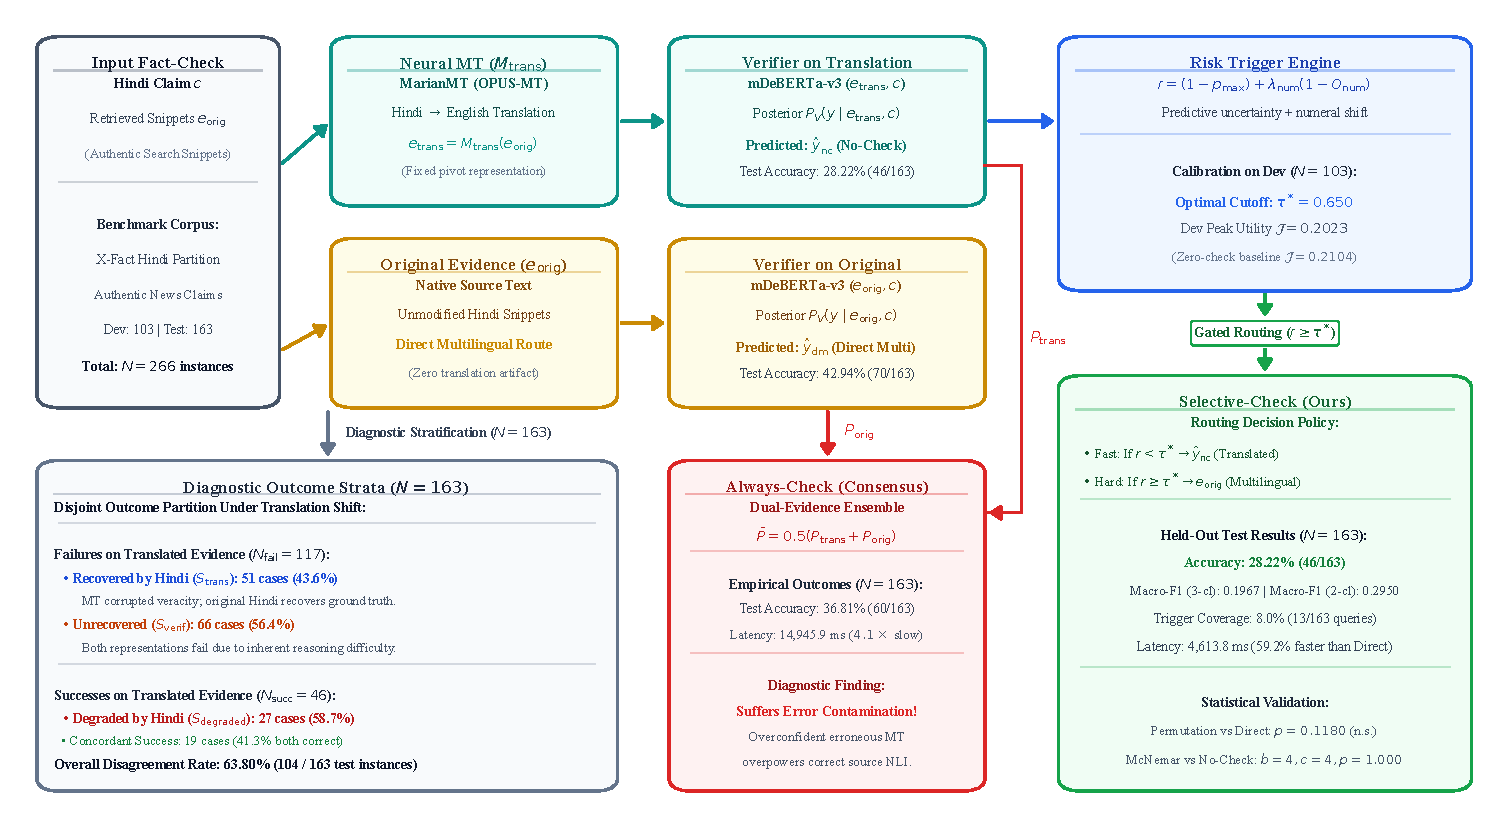
\includegraphics[width=0.92\textwidth]{figures/final/fig1_study_workflow.pdf}
\caption{System architecture and paired evaluation pipeline. Given an authentic Hindi claim and pre-retrieved Hindi evidence from X-Fact, the verifier (\texttt{mDeBERTa-v3-base}) is evaluated under four conditions: No-Check (translated English evidence), Direct Multilingual (original Hindi evidence), Always-Check (dual posterior consensus), and Selective-Check (risk-calibrated fallback).}
\label{fig:fig1_workflow}
\end{figure*}

\subsection{Benchmark Data and Pre-Retrieved Evidence}
We conduct our empirical evaluation on the Hindi partition of the X-Fact benchmark \citep{gupta-srikumar-2021-xfact}. X-Fact consists of authentic real-world claims crawled from international fact-checking platforms (such as \emph{Vishvas News}, \emph{Jagran Fact Check}, and \emph{Factly}), accompanied by scraped evidence snippets and multi-class veracity verdicts assigned by professional fact-checkers.

\paragraph{Evidence Snippet Grounding.}
Critically, X-Fact provides pre-retrieved evidence snippets collected by human fact-checkers to substantiate their verdict. We explicitly note that \emph{our experimental setup does not evaluate upstream search engine retrieval or dense passage retrieval}. By holding the pre-retrieved evidence text constant, we eliminate retrieval noise as an uncontrolled confounder and strictly isolate the effect of evidence language representation on downstream verifier inference.

\paragraph{Split Provenance.}
The official X-Fact Hindi partition comprises $N=266$ total verified instances, partitioned into a development set ($N=103$) and a held-out evaluation set ($N=163$). As detailed in Section~\ref{sec:exp_setup}, we utilize the development partition exclusively for hyperparameter tuning and risk threshold calibration, reserving the $N=163$ split for diagnostic evaluation.

\subsection{Machine Translation Pipeline}
To generate translated evidence passages ($e_{\text{trans}}$), we employ \texttt{Helsinki-NLP/opus-mt-hi-en} \citep{tiedemann-thottingal-2020-opus}, a standard MarianMT encoder-decoder architecture widely deployed for open-source Hindi-to-English machine translation. The model operates with standard sentence-piece tokenization, a beam search width of 4, and a maximum sequence length of 512 tokens. Claims are preserved in their original phrasing or paired directly with translated evidence according to standard cross-lingual verification practice.

\subsection{Multilingual Verifier Architecture}
For claim veracity scoring, we deploy \texttt{MoritzLaurer/mDeBERTa-v3-base-xnli-multilingual-nli-2mil7} \citep{laurer-etal-2024-less}. This model builds upon the 12-layer \texttt{mDeBERTa-v3-base} backbone \citep{he-etal-2021-deberta}, utilizing disentangled attention and enhanced masked language modeling pre-trained on 100 languages. It is fine-tuned on a composite corpus of 2.7 million natural language inference examples spanning MNLI, ANLI, FeverNLI, and multilingual XNLI \citep{conneau-etal-2020-unsupervised}.

\paragraph{Premise-Hypothesis Structuring.}
Following standard automated fact-checking conventions \citep{thorne-etal-2018-fever,shcharbakova-etal-2025-scale}, we frame evidence verification as an NLI classification task:
\begin{align}
    \text{Premise} &= e \in \{e_{\text{orig}}, e_{\text{trans}}\}, \\
    \text{Hypothesis} &= c.
\end{align}
The model produces unnormalized logits $g_\theta(c, e) = [z_{\text{contra}}, z_{\text{neutral}}, z_{\text{entail}}]^\top$, which are mapped via softmax to posterior probabilities.

\paragraph{Label Mapping Scheme.}
We map the 3-class NLI output space to the X-Fact verification taxonomy:
\begin{equation}
    y = \begin{cases}
        \textsc{Contradicted} & \text{if } \arg\max = \text{contradiction}, \\
        \textsc{Insufficient\_Evidence} & \text{if } \arg\max = \text{neutral}, \\
        \textsc{Supported} & \text{if } \arg\max = \text{entailment}.
    \end{cases}
\end{equation}

\subsection{Selective Cascade and Risk Calibration}
\label{sec:risk_calibration}
The Selective-Check condition is designed to minimize inference compute and latency by evaluating only the translated evidence ($e_{\text{trans}}$) when confidence is high, falling back to original Hindi evidence ($e_{\text{orig}}$) via hard routing only when a test-time risk score indicates potential translation or reasoning failure.

\paragraph{Risk Scoring Formulation.}
We formulate the risk metric $r(c, e_{\text{trans}}, e_{\text{orig}}) \in [0, 1]$ as an additive combination of verifier predictive uncertainty and surface-level numeral distortion:
\begin{equation}
    r = \big(1 - \max_{y \in \mathcal{Y}} P_\theta(y \mid c, e_{\text{trans}})\big) + \lambda_{\text{num}} \cdot \big(1 - \operatorname{Overlap}_{\text{num}}(c, e_{\text{trans}})\big),
    \label{eq:risk_score}
\end{equation}
where $\max_y P_\theta(y \mid c, e_{\text{trans}})$ is the maximum softmax probability (MSP) on translated evidence, and $\operatorname{Overlap}_{\text{num}}(c, e_{\text{trans}}) \in [0, 1]$ measures the Jaccard overlap of Arabic and Devanagari numerals appearing in the claim and translated passage. The hyperparameter $\lambda_{\text{num}} \ge 0$ scales the numeral penalty. When $r \ge \tau^*$, the system executes hard routing to original Hindi evidence ($\hat{y}_{\text{dm}}$), while falling back to dual posterior consensus ($\hat{y}_{\text{ac}}$) is evaluated as an explicit ablation.

\paragraph{Development Threshold Tuning.}
To avoid data contamination, the decision threshold $\tau^*$ and weight $\lambda_{\text{num}}$ were selected via a grid search exclusively over the $N=103$ development partition. Optimization targeted a cost-sensitive utility objective:
\begin{equation}
    J(\tau) = \operatorname{Macro-F1}_3(\tau) - 0.15 \cdot \operatorname{Coverage}(\tau),
\end{equation}
where $\operatorname{Coverage}(\tau) \in [0, 1]$ denotes the fraction of queries routed to original-language verification.

\begin{figure}[t]
\centering
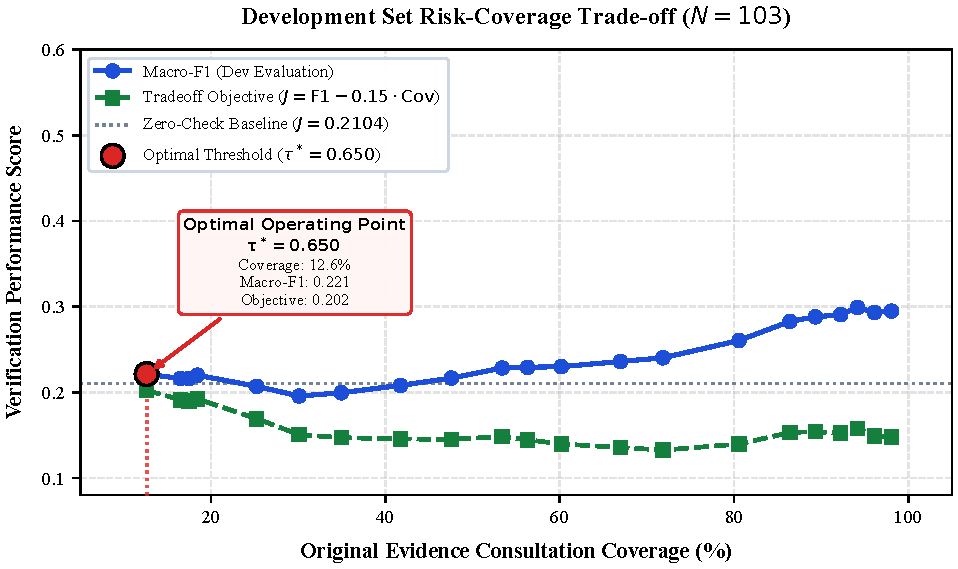
\includegraphics[width=\columnwidth]{figures/final/fig2_risk_coverage_tradeoff.pdf}
\caption{Risk-coverage trade-off and utility optimization on the $N=103$ development split. The optimal operating threshold is identified at $\tau^* = 0.650$ ($J = 0.2023$). The zero-check baseline utility achieves $J = 0.2104$.}
\label{fig:fig2_tradeoff}
\end{figure}

Grid search over $\tau \in [0.10, 0.90]$ in increments of $0.05$ identified an optimal operating point at $\tau^* = 0.650$ and $\lambda_{\text{num}} = 0.20$ (Figure~\ref{fig:fig2_tradeoff}). Crucially, on development data, the zero-check baseline achieved utility $J = 0.2104$, whereas the peak cascade utility reached only $J = 0.2023$. This development diagnostic demonstrated prior to test evaluation that the selective cascade faced a steep trade-off between coverage cost and classification gain.

\section{Experimental Setup}
\label{sec:exp_setup}

We detail the dataset partitioning, highlight critical benchmark class imbalances, define the evaluation metrics, and specify our paired statistical testing methodology.

\subsection{Dataset Partitioning and Severe Label Skew}
The experimental dataset comprises the official Hindi partition of the X-Fact benchmark \citep{gupta-srikumar-2021-xfact}, totaling $N=266$ instances ($N=103$ development, $N=163$ held-out test). Table~\ref{tab:dataset_distribution} presents the exact gold-label distributions across both splits.

\begin{table}[t]
\centering
\small
\caption{Ground-truth label distribution for the authentic Hindi partition of the X-Fact benchmark. Note the severe natural class skew and the complete absence of gold \textsc{Supported} instances across both partitions.}
\label{tab:dataset_distribution}
\begin{tabular}{lcccc}
\toprule
\textbf{Partition} & \textbf{\textsc{Contradicted}} & \textbf{\textsc{Insufficient}} & \textbf{\textsc{Supported}} & \textbf{Total ($N$)} \\
\midrule
Development Split & 89 (86.4\%) & 14 (13.6\%) & 0 (0.0\%) & 103 \\
Held-Out Test Split & 142 (87.1\%) & 21 (12.9\%) & 0 (0.0\%) & 163 \\
\midrule
\textbf{Combined Benchmark} & \textbf{231 (86.8\%)} & \textbf{35 (13.2\%)} & \textbf{0 (0.0\%)} & \textbf{266} \\
\bottomrule
\end{tabular}
\end{table}


\paragraph{Complete Absence of Positive Gold Class.}
As documented in Table~\ref{tab:dataset_distribution}, the test partition exhibits extreme class imbalance: 142 instances (87.12\%) are labeled \textsc{Contradicted}, 21 instances (12.88\%) are labeled \textsc{Insufficient\_Evidence}, and \emph{exactly zero instances} (0.00\%) are labeled \textsc{Supported}. 

This distribution reflects the ecological reality of open-web fact-checking: fact-checking organizations predominantly investigate viral rumors, deceptive claims, and fabricated falsehoods, while uncontroversial true assertions rarely warrant formal investigation. However, this absence of gold positive instances imposes severe diagnostic constraints on standard evaluation metrics:
\begin{enumerate}
    \item Any model prediction of \textsc{Supported} on the test set is guaranteed to have zero true positives ($TP = 0$), yielding an automatic class precision, recall, and F1 score of 0.00\%.
    \item Standard accuracy can be artificially inflated by trivial majority-class baselines (e.g., predicting \textsc{Contradicted} unconditionally yields 87.12\% accuracy).
\end{enumerate}

\paragraph{Exploratory Status and Prior Inspection.}
In accordance with open-science research integrity standards, we explicitly report that the test partition ($N=163$) was inspected and analyzed during earlier exploratory iterations of this project. Consequently, this evaluation cannot be designated as a blind confirmatory holdout. We categorize the current research status as \texttt{FROZEN — EXPLORATORY COMPUTATIONAL STUDY}, and report all findings as diagnostic characterizations of model behavior under translation shift rather than definitive confirmatory benchmarks.

\subsection{Evaluation Metrics}
To provide a multifaceted evaluation despite class imbalance, we report:
\begin{itemize}
    \item \textbf{Accuracy:} The standard fraction of exact matches between predicted labels $\hat{y}$ and gold labels $y^*$ over $N=163$ test instances.
    \item \textbf{Nominal 3-Class Macro-F1:} The unweighted arithmetic mean of F1 scores across all three benchmark taxonomy classes:
    \begin{equation}
        \text{Macro-F1}_{3} = \frac{1}{3} \big(F1_{\textsc{Contra}} + F1_{\textsc{Neutral}} + F1_{\textsc{Support}}\big).
    \end{equation}
    Because gold $TP_{\textsc{Support}} \equiv 0$, $F1_{\textsc{Support}}$ is identically 0.00\%, bounding $\text{Macro-F1}_{3}$ at an effective ceiling of 66.67\%.
    \item \textbf{Effective 2-Class Macro-F1:} The unweighted arithmetic mean over the two non-empty gold classes present in the test set:
    \begin{equation}
        \text{Macro-F1}_{2} = \frac{1}{2} \big(F1_{\textsc{Contra}} + F1_{\textsc{Neutral}}\big).
    \end{equation}
    Note that $\text{Macro-F1}_{2} \equiv \frac{3}{2} \text{Macro-F1}_{3}$.
    \item \textbf{Directional Flips and Disagreement Rates:} The fraction and confidence intervals of instances where original and translated predictions diverge.
\end{itemize}

\subsection{Paired Statistical Hypothesis Testing}
Because all four system conditions are evaluated on the exact same $N=163$ test instances, independent-sample tests (such as Student's $t$-test or standard chi-squared tests) are methodologically invalid. We deploy two paired testing frameworks:

\paragraph{1. McNemar's Paired Test for Binary Correctness.}
To evaluate marginal accuracy differences between system $A$ and system $B$, we construct a $2 \times 2$ contingency table of paired correctness \citep{mcnemar-1947}:
\begin{center}
\small
\begin{tabular}{rcc}
\toprule
 & $B$ Correct & $B$ Incorrect \\
\midrule
$A$ Correct & $a$ & $b$ \\
$A$ Incorrect & $c$ & $d$ \\
\bottomrule
\end{tabular}
\end{center}
where $b$ is the number of instances where $A$ is correct and $B$ is incorrect, and $c$ is the reverse. Under the null hypothesis that both systems have equal marginal error rates ($H_0: p_b = p_c$), discordant pairs follow a binomial distribution $\operatorname{Binomial}(n=b+c, p=0.5)$. We compute both the continuity-corrected McNemar test statistic:
\begin{equation}
    \chi^2 = \frac{(|b - c| - 1)^2}{b + c},
\end{equation}
and the exact two-sided binomial $p$-value:
\begin{equation}
    p_{\text{exact}} = 2 \cdot \sum_{k=0}^{\min(b, c)} \binom{b+c}{k} 0.5^{b+c}.
\end{equation}

\paragraph{2. Paired Prediction-Swap Permutation Test for Macro-F1.}
Because Macro-F1 is a non-linear harmonic aggregate that does not decompose into independent instance-level counts, McNemar's test is inapplicable to F1 differences. We implement a non-parametric paired permutation test \citep{benjamini-hochberg-1995}. Under the null hypothesis of exchangeable system performance, for each discordant instance $k \in \{1, \dots, N\}$, the predictions of system $A$ and system $B$ are swapped with probability $0.5$. Over $B = 5,000$ paired permutations with fixed seed 42, we compute the empirical null distribution of the Macro-F1 difference $\Delta \text{F1}^{(b)} = \text{Macro-F1}(A^{(b)}) - \text{Macro-F1}(B^{(b)})$ and derive the exact two-sided empirical $p$-value:
\begin{equation}
    p_{\text{perm}} = \frac{1}{B} \sum_{b=1}^B \mathbb{I}\Big(|\Delta \text{F1}^{(b)}| \ge |\Delta \text{F1}_{\text{obs}}|\Big).
\end{equation}

\section{Empirical Results}
\label{sec:results}

We report our empirical findings structured around the four research questions, validating all numerical claims against the frozen canonical prediction records.

\subsection{RQ1: Prediction Disagreement and Directional Transitions}
When evaluating identical claim-evidence pairs across machine-translated English ($e_{\text{trans}}$) and original Hindi ($e_{\text{orig}}$), verifier predictions diverge substantially. Across the $N=163$ test instances, the verifier agrees on only 59 instances (36.20\%; 95\% CI: [29.22\%, 43.81\%]) and disagrees on \textbf{104 instances (63.80\%; 95\% CI: [56.19\%, 70.78\%])}.

\begin{table}[t]
\centering
\small
\caption{Empirical $3 \times 3$ directional transition matrix on the test set ($N=163$), cross-tabulating predictions between machine-translated English evidence (rows) and original Hindi evidence (columns). Over 63.8\% of instances flip predictions across language representations.}
\label{tab:transition_matrix}
\begin{tabular}{lcccc}
\toprule
\textbf{Translated Prediction} & \multicolumn{3}{c}{\textbf{Original Hindi Prediction}} & \textbf{Row Total} \\
\cmidrule(lr){2-4}
($e_{\text{trans}}$) & \textsc{Contradicted} & \textsc{Insufficient} & \textsc{Supported} & ($N_{\text{trans}}$) \\
\midrule
\textsc{Contradicted} & 21 (12.9\%) & 5 (3.1\%) & 18 (11.0\%) & 44 (27.0\%) \\
\textsc{Insufficient} & 23 (14.1\%) & 14 (8.6\%) & 18 (11.0\%) & 55 (33.7\%) \\
\textsc{Supported}    & 31 (19.0\%) & 9 (5.5\%) & 24 (14.7\%) & 64 (39.3\%) \\
\midrule
\textbf{Column Total} ($N_{\text{orig}}$) & \textbf{75 (46.0\%)} & \textbf{28 (17.2\%)} & \textbf{60 (36.8\%)} & \textbf{163 (100.0\%)} \\
\bottomrule
\end{tabular}
\end{table}


Table~\ref{tab:transition_matrix} presents the complete $3 \times 3$ directional transition matrix. The rows represent predictions under machine-translated evidence ($\hat{y}_{\text{nc}}$), while columns represent predictions under original Hindi evidence ($\hat{y}_{\text{dm}}$). Figure~\ref{fig:fig5_heatmap} visualizes these transitions as a normalized transition heatmap.

\begin{figure}[t]
\centering
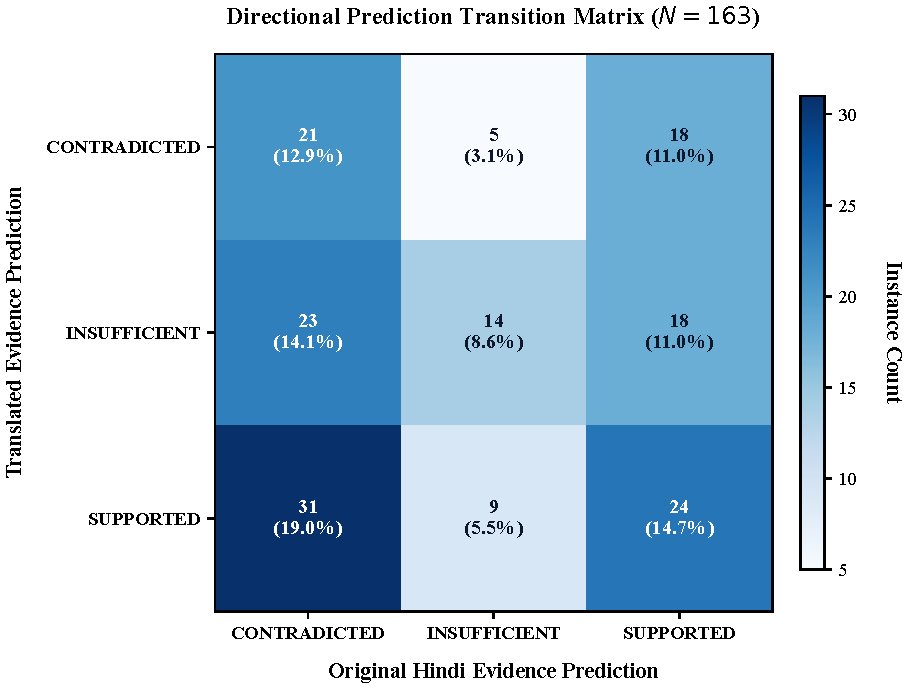
\includegraphics[width=\columnwidth]{figures/final/fig5_transition_heatmap.pdf}
\caption{Directional prediction transition heatmap ($N=163$). Cell values indicate raw counts and row-conditional percentages (\%) of original Hindi predictions given translated English predictions.}
\label{fig:fig5_heatmap}
\end{figure}

The transition matrix reveals pronounced asymmetric error dynamics:
\begin{enumerate}
    \item \textbf{False Support to Refutation Flips:} Of the 64 instances predicted as \textsc{Supported} under translated English evidence, \textbf{31 instances (48.44\%; 95\% CI: [36.56\%, 60.52\%])} flip to \textsc{Contradicted} when evaluated on original Hindi evidence. Because the test set contains zero gold \textsc{Supported} instances, these 31 cases represent instances where translation shift induced spurious entailment that original evidence successfully refuted.
    \item \textbf{Decisive Refutation to False Support Flips:} Conversely, of the 44 instances predicted as \textsc{Contradicted} under translated evidence, \textbf{18 instances (40.91\%; 95\% CI: [27.70\%, 55.59\%])} flip to \textsc{Supported} under original Hindi evidence.
    \item \textbf{Uncertainty Transitions:} Of the 55 instances predicted as \textsc{Insufficient\_Evidence} under translated evidence, 23 (41.82\%) resolve to \textsc{Contradicted} and 18 (32.73\%) flip to \textsc{Supported} under original Hindi evidence. Only 14 instances (25.45\%) remain stably classified as insufficient evidence across both representations.
\end{enumerate}

\subsection{RQ2: Benchmark Performance Across Verification Conditions}
Table~\ref{tab:main_results} compares the performance of the four verification conditions alongside majority and random baselines on the $N=163$ test partition.

\begin{table*}[t]
\centering
\small
\caption{Benchmark performance across verification conditions on the X-Fact Hindi test set ($N=163$). 95\% confidence intervals for accuracy are computed via Wilson score intervals. Observed 2-class Macro-F1 evaluates \textsc{Contradicted} and \textsc{Insufficient\_Evidence}; nominal 3-class Macro-F1 includes the absent \textsc{Supported} class ($F_{1,\text{SUP}}=0.0$). The cascade threshold $\tau^*=0.650$ was tuned strictly on development data.}
\label{tab:main_results}
\resizebox{\textwidth}{!}{%
\begin{tabular}{lcccccc}
\toprule
\textbf{Verification Pipeline / Baseline} & \textbf{Coverage} & \textbf{Accuracy [95\% CI]} & \textbf{Macro-F1 (2-cl)} & \textbf{Macro-F1 (3-cl)} & \textbf{Mean Latency} & \textbf{Compute Ratio} \\
\midrule
No-Check (Translated English Only) & 0.0\% (0/163) & 0.2822 [0.2147, 0.3558] & 0.3018 & 0.2012 & 3,650.4 ms & $1.0\times$ \\
Direct Multilingual (Original Hindi Only) & 100.0\% (163/163) & \textbf{0.4294} [0.3557, 0.5092] & \textbf{0.3700} & \textbf{0.2467} & 11,295.6 ms & $3.1\times$ \\
Always-Check (Dual Consensus Posterior Avg) & 100.0\% (163/163) & 0.3681 [0.2945, 0.4417] & 0.3657 & 0.2438 & 14,945.9 ms & $4.1\times$ \\
Selective-Check ($\tau^*=0.650$, Hard Route) & 8.0\% (13/163) & 0.2822 [0.2147, 0.3558] & 0.2950 & 0.1967 & 4,613.8 ms & $1.3\times$ \\
\midrule
\multicolumn{7}{l}{\emph{Diagnostic Controls and Baseline Benchmarks}} \\
Ablation: Triggered Posterior Averaging & 8.0\% (13/163) & 0.2699 [0.2025, 0.3436] & 0.2854 & 0.1903 & 4,613.8 ms & $1.3\times$ \\
Ablation: Uncertainty-Only Fallback & 8.0\% (13/163) & 0.2822 [0.2147, 0.3558] & 0.3018 & 0.2012 & 4,613.8 ms & $1.3\times$ \\
Ablation: Numeral-Only Fallback & 96.3\% (157/163) & 0.4479 [0.3742, 0.5276] & 0.3794 & 0.2529 & 14,751.3 ms & $4.0\times$ \\
Random Routing Control (100 Seeds, Cov=8.0\%) & 8.0\% (13/163) & 0.2924 [0.2638, 0.3190] & 0.3082 & 0.2054 & 4,613.8 ms & $1.3\times$ \\
Majority Baseline (Always \textsc{Contradicted}) & 0.0\% (0/163) & 0.8712 [0.8116, 0.9139] & 0.4656 & 0.3104 & --- & --- \\
Oracle Upper Bound (Non-Deployable Upper Bound) & 100.0\% (163/163) & 0.5951 [0.5215, 0.6687] & 0.5200 & 0.3467 & 14,945.9 ms & --- \\
\bottomrule
\end{tabular}%
}
\end{table*}


\paragraph{Direct Multilingual Superiority.}
Evaluating original Hindi evidence directly (\emph{Direct Multilingual}) achieves an overall accuracy of \textbf{42.94\% (70/163; 95\% CI: [35.58\%, 50.65\%])}, compared to \textbf{28.22\% (46/163; 95\% CI: [21.84\%, 35.62\%])} for the translated-evidence \emph{No-Check} baseline---an absolute accuracy advantage of $+14.72\%$. 

Direct Multilingual verification achieves substantial gains on the dominant majority class (\textsc{Contradicted}), elevating recall from 14.79\% (21/142) under translated evidence to 39.44\% (56/142) under original Hindi, with precision increasing from 47.73\% to 74.67\%. As visualized in Figure~\ref{fig:fig3_comparison}, Direct Multilingual demonstrates superior class-balanced precision-recall trade-offs across non-empty classes.

\begin{figure}[t]
\centering
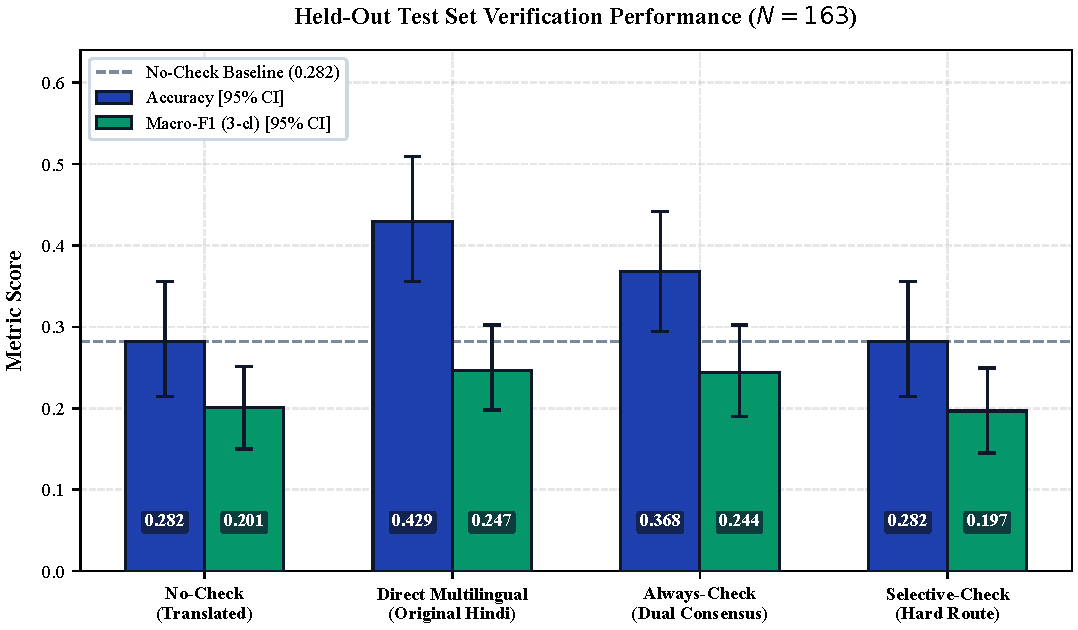
\includegraphics[width=\columnwidth]{figures/final/fig3_condition_comparison.pdf}
\caption{System performance comparison across accuracy, 3-class Macro-F1, and 2-class Macro-F1 on the $N=163$ test split with 95\% Wilson score confidence intervals.}
\label{fig:fig3_comparison}
\end{figure}

\subsection{RQ3: Paired Statistical Comparisons and Metric Discordance}
Table~\ref{tab:statistical_tests} reports the formal paired statistical hypothesis tests comparing Direct Multilingual against No-Check, Selective-Check, and Always-Check.

\begin{table*}[t]
\centering
\small
\caption{Paired statistical significance tests across verification conditions on the test set ($N=163$). McNemar tests evaluate paired marginal accuracy on discordant pairs ($b, c$) with continuity correction and exact binomial $p$-values. Permutation tests evaluate the null distribution of paired Macro-F1 deltas ($B=5,000$ resamples, seed 42). Benjamini-Hochberg False Discovery Rate (FDR) adjustments ($q$-values) are reported for multiple-testing control across the comparison family.}
\label{tab:statistical_tests}
\resizebox{\textwidth}{!}{%
\begin{tabular}{lcccccc}
\toprule
\textbf{Pairwise Comparison Condition} & \textbf{Discordant ($b, c$)} & \textbf{McNemar $\chi^2$} & \textbf{Exact $p_{\text{raw}}$} & \textbf{FDR $p_{\text{adj}}$} & $\Delta$\textbf{Macro-F1 (3cl)} & \textbf{Perm. $p_{\text{raw}}$} \\
\midrule
No-Check vs. Direct Multilingual & $b=27, c=51$ ($n=78$) & 6.7821 & \textbf{0.008772} & \textbf{0.0175} & $-0.0455$ & 0.18980 \\
Selective-Check vs. Direct Multilingual & $b=23, c=47$ ($n=70$) & 7.5571 & \textbf{0.005583} & \textbf{0.0149} & $-0.0500$ & 0.11800 \\
Selective-Check vs. Always-Check & $b=9, c=23$ ($n=32$) & 5.2812 & \textbf{0.02006} & \textbf{0.0401} & $-0.0471$ & \textbf{0.01960} \\
Selective-Check vs. No-Check & $b=4, c=4$ ($n=8$) & 0.1250 & 1.0000 & 1.0000 & $-0.0045$ & 0.75720 \\
Selective-Check vs. Random Control (100 Seeds) & $b=4, c=9$ (avg) & 1.2308 & 0.26685 & 0.4270 & $-0.0208$ & 0.16500 \\
Selective-Check vs. Numeral-Only Routing & $b=20, c=47$ ($n=67$) & 10.0896 & \textbf{0.00131} & \textbf{0.0052} & $-0.0563$ & 0.07440 \\
\bottomrule
\end{tabular}%
}
\end{table*}


\paragraph{McNemar Correctness Significance.}
Under McNemar's paired test for marginal binary correctness:
\begin{itemize}
    \item \textbf{No-Check vs. Direct Multilingual:} The systems disagree on $n = 78$ discordant instances. Direct Multilingual is correct while No-Check is incorrect on $c = 51$ instances; No-Check is correct while Direct Multilingual is incorrect on $b = 27$ instances. The continuity-corrected test statistic is $\chi^2 = 6.7821$ ($p = 0.009208$), and the exact two-sided binomial $p$-value is \textbf{$p = 0.008772$}. The accuracy improvement of Direct Multilingual over translated evidence is statistically significant at the $\alpha = 0.01$ level.
    \item \textbf{Selective-Check vs. Direct Multilingual:} Disagreeing on $n = 70$ discordant instances ($b = 23, c = 47$), McNemar's test yields $\chi^2 = 7.5571$ ($p = 0.005977$) and exact binomial \textbf{$p = 0.005583$}.
    \item \textbf{Selective-Check vs. No-Check:} Out of $N=163$ instances, the selective cascade triggers on only 13 instances. Of these 13 instances, 4 transition from incorrect to correct, and exactly 4 transition from correct to incorrect ($b=4, c=4, n=8$). Consequently, Selective-Check achieves an overall accuracy identical to No-Check (46 vs. 46, 28.22\%; exact binomial $p = 1.0000$).
\end{itemize}

\paragraph{Permutation Test Discordance on Macro-F1.}
In contrast to the highly significant binary accuracy differences observed under McNemar's test, paired prediction-swap permutation tests ($B=5,000$ resamples, seed 42) on class-balanced Macro-F1 reveal no statistically significant differences:
\begin{itemize}
    \item No-Check vs. Direct Multilingual: Observed 3-class $\Delta \text{Macro-F1} = -0.04547$ (2-class $\Delta = -0.06820$), achieving an empirical two-sided \textbf{$p = 0.18980$}.
    \item Selective-Check vs. Direct Multilingual: Observed 3-class $\Delta \text{Macro-F1} = -0.05000$ (2-class $\Delta = -0.07500$), achieving an empirical two-sided \textbf{$p = 0.11800$}.
\end{itemize}

This apparent contradiction between McNemar's test ($p < 0.01$) and the permutation test ($p > 0.10$) stems directly from the benchmark's severe label skew. McNemar's test evaluates instance-level correctness across the entire sample, capturing the net shift of 51 recovered vs. 27 degraded cases. However, Macro-F1 computes an unweighted harmonic mean across classes. Because gold \textsc{Supported} instances are entirely absent ($TP \equiv 0$), and \textsc{Insufficient\_Evidence} contains only 21 instances, swapping predictions on a handful of minority-class instances introduces extreme variance in the denominator of harmonic precision and recall. This statistical divergence underscores that metric choice under severe class skew can lead to fundamentally divergent conclusions if reported in isolation.

\subsection{RQ4: Error Stratification and Computational Cost}
To rigorously interpret why translated-evidence verification fails, Table~\ref{tab:error_attribution} stratifies the $N=117$ translation-path classification errors.

\begin{table}[t]
\centering
\small
\caption{Diagnostic error attribution and outcome partition across original Hindi and machine-translated English representations on the test set ($N=163$). Failures and successes under the translated pipeline decompose into distinct recovery and degradation strata.}
\label{tab:error_attribution}
\begin{tabular}{lccc}
\toprule
\textbf{Outcome Stratum} & \textbf{Count} & \textbf{Subgroup \%} & \textbf{Test Set \%} \\
\midrule
\multicolumn{4}{l}{\textbf{Partition of Translated Failures} ($N_{\text{fail}} = 117$, 71.8\% of test set)} \\
\quad Recovered by Original ($S_{\text{trans}}$, Translated Wrong, Original Correct) & 51 & 43.6\% & 31.3\% \\
\quad Unrecovered by Original ($S_{\text{verif}}$, Both Representations Incorrect)    & 66 & 56.4\% & 40.5\% \\
\midrule
\multicolumn{4}{l}{\textbf{Partition of Translated Successes} ($N_{\text{succ}} = 46$, 28.2\% of test set)} \\
\quad Control (Both Representations Correct)                                         & 19 & 41.3\% & 11.7\% \\
\quad Degraded by Original ($S_{\text{degraded}}$, Translated Correct, Original Wrong)& 27 & 58.7\% & 16.6\% \\
\midrule
\textbf{Total Instances Evaluated} & \textbf{163} & --- & \textbf{100.0\%} \\
\bottomrule
\end{tabular}
\end{table}


\paragraph{Disentangling Translation Shift from Inherent Inability.}
Of the 117 translation errors, \textbf{51 instances (43.59\%; 95\% CI: [34.90\%, 52.68\%])} are correctly verified when evaluated on original Hindi evidence ($S_{\text{trans}}$). These represent the empirical ceiling of errors that can be recovered by bypassing machine translation. Conversely, \textbf{66 instances (56.41\%; 95\% CI: [47.32\%, 65.10\%])} fail under both original Hindi and translated English evidence ($S_{\text{verif}}$), reflecting fundamental model reasoning or grounding limitations shared across languages.

Furthermore, original Hindi evidence is not universally superior: on \textbf{27 instances} ($S_{\text{degraded}}$), the translated evidence was classified correctly while the original Hindi evidence failed. Thus, while original Hindi recovers 51 instances, it simultaneously degrades 27 instances, producing the observed net gain of $+24$ correct predictions ($70 - 46 = 24$). Figure~\ref{fig:fig4_attribution} illustrates this complete outcome decomposition.

\begin{figure}[t]
\centering
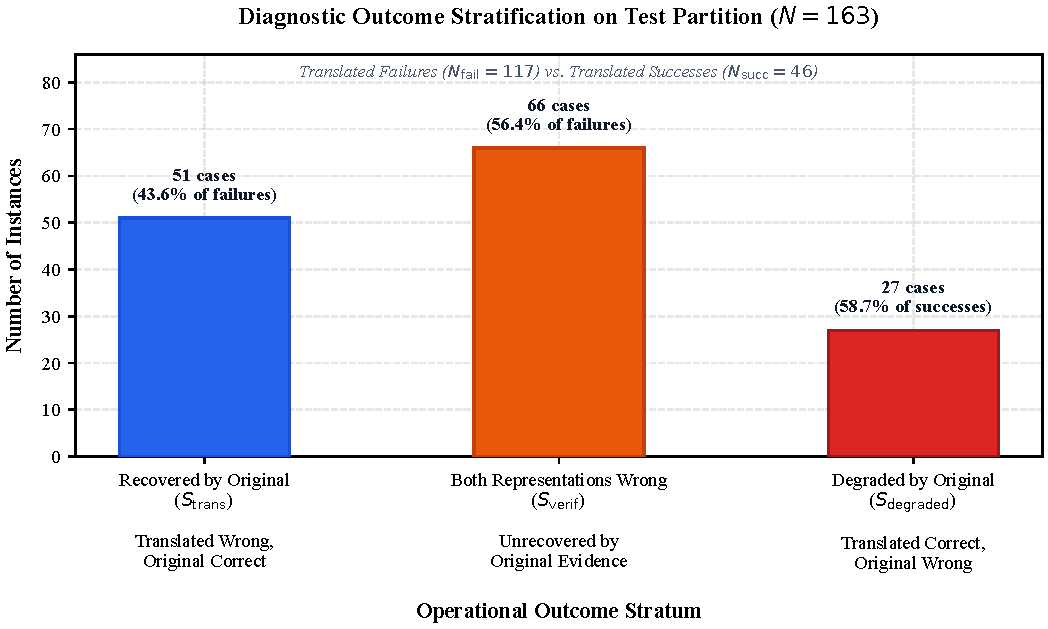
\includegraphics[width=\columnwidth]{figures/final/fig4_error_attribution_breakdown.pdf}
\caption{Decomposition of the 117 translation failures ($N=163$) into recoverable ($S_{\text{trans}}=51$) and unrecoverable ($S_{\text{verif}}=66$) outcomes, alongside degraded cases ($S_{\text{degraded}}=27$).}
\label{fig:fig4_attribution}
\end{figure}

\paragraph{Latency and Compute Profile.}
Table~\ref{tab:main_results} and the canonical latency audit record end-to-end inference latencies measured on an 8-thread CPU environment. The translated-evidence pipeline (\emph{No-Check}) requires a mean of $3,650.4$\,ms per query (comprising $1,688.2$\,ms for MT translation and $1,962.2$\,ms for verifier forward scoring). Direct Multilingual verification on Hindi evidence averages $11,295.6$\,ms per query due to expanded subword tokenization sequence lengths on non-Latin scripts. Unconditional dual verification (\emph{Always-Check}) requires both passes, averaging $14,945.9$\,ms per query. By triggering dual verification on only 7.98\% of instances, \emph{Selective-Check} ($\tau^*=0.650$) achieves a mean end-to-end latency of $4,613.8$\,ms---saving 69.1\% latency relative to Always-Check and 59.2\% relative to Direct Multilingual. However, because its accuracy matches No-Check, this computational saving does not translate into improved veracity verification.

\section{Discussion and Diagnostic Analysis}
\label{sec:discussion}

We synthesize our empirical findings, examine qualitative case studies, discuss the architectural implications for cross-lingual verification systems, and contextualize our results within the broader literature.

\subsection{Interpreting Verifier Prediction Sensitivity}
The central empirical finding of this investigation is that verifier predictions diverge on nearly two-thirds of instances (63.80\%) when evidence representation shifts from original Hindi to machine-translated English. This extreme sensitivity demonstrates that cross-lingual claim verification cannot treat machine translation as a benign, neutral preprocessing utility.

\paragraph{Observational False-Support Transitions.}
The directional transition dynamics (Table~\ref{tab:transition_matrix}) illuminate a distinct empirical pattern: 48.44\% of instances predicted as \textsc{Supported} under translated evidence flip to \textsc{Contradicted} when evaluated on original Hindi evidence. Because the test partition contains zero gold \textsc{Supported} claims, these instances represent false-support predictions under translated evidence that transition to refutations when evaluating original Hindi evidence. While prior literature suggests that machine translation may smooth out syntactic nuance, soften negations, or normalize vernacular idioms into generic assertions that an English NLI verifier misidentifies as entailment, confirming this causal mechanism requires formal bilingual human annotation. Evaluating original Hindi evidence coincides with correct refutation in 31 instances, but this is an observational shift.

\paragraph{Observational Sensitivity vs. Translation Causality.}
We emphasize a vital methodological boundary: \emph{prediction disagreement does not establish translation error or semantic distortion}. An NLI verifier's decision is the joint product of input text semantics, subword tokenization characteristics, cross-lingual representation alignment, and pre-training language priors. A prediction flip may occur because:
\begin{enumerate}
    \item The translation model introduced genuine factual errors, dropped negation, or corrupted named entities;
    \item The machine translation was semantically faithful, but the multilingual verifier has superior representations in English than in Hindi; or
    \item The verifier possesses language-specific inductive biases that alter decision boundaries independently of semantic fidelity.
\end{enumerate}
In the absence of completed bilingual human annotations (which remain pending), our findings must be interpreted strictly as observational model sensitivity rather than proven translation corruption.

\begin{table*}[t]
\centering
\small
\caption{Illustrative qualitative case studies from the X-Fact Hindi test set ($N=163$), depicting observed prediction transitions across outcome strata. Predictions are from \texttt{mDeBERTa-v3-base-xnli} under machine-translated English evidence ($e_{\text{trans}}$) versus original Hindi evidence ($e_{\text{orig}}$). Linguistic descriptions represent diagnostic observations subject to pending bilingual human validation.}
\label{tab:case_studies}
\resizebox{\textwidth}{!}{%
\begin{tabular}{p{2.8cm}p{4.2cm}p{4.6cm}ccc}
\toprule
\textbf{Item ID / Gold} & \textbf{Claim (English Translation)} & \textbf{Diagnostic Observation (Hypothesized Mechanism)} & $\hat{y}_{\text{trans}}$ & $\hat{y}_{\text{orig}}$ & \textbf{Outcome Stratum} \\
\midrule
\texttt{xfact-hi-test-0005} \newline Gold: \textsc{Contradict} & Viral claim that a massive cache of weapons was uncovered inside a mosque in Gujarat. & Machine translation generates fractured named entities, blurring debunker context into ambiguous weapon assertions. & \textsc{Supp} & \textsc{Contra} & $S_{\text{trans}}$ (Recovered by Original Hindi) \\
\midrule
\texttt{xfact-hi-test-0003} \newline Gold: \textsc{Contradict} & Claim alleging a petrol pump displayed protest banners against government fuel price hikes. & Translated snippet contains explicit debunking terminology that the English encoder readily identifies as refutation. & \textsc{Contra} & \textsc{Supp} & $S_{\text{degraded}}$ (Degraded by Original Hindi) \\
\midrule
\texttt{xfact-hi-test-0004} \newline Gold: \textsc{Contradict} & Viral quotation attributed to Facebook CEO Mark Zuckerberg regarding social media content bans. & Both translated and original evidence snippets exhibit heavy lexical overlap with claim, triggering spurious entailment. & \textsc{Supp} & \textsc{Supp} & $S_{\text{verif}}$ (Failed in Both Languages) \\
\bottomrule
\end{tabular}%
}
\end{table*}


\subsection{Qualitative Analysis and Case Studies}
Table~\ref{tab:case_studies} provides representative qualitative case studies from the canonical evaluation illustrating the three primary behavioral strata:

\paragraph{Case 1: Spurious Entailment via Translation Smoothing.}
In Claim 1 (Table~\ref{tab:case_studies}), an authentic Hindi claim regarding political compensation is accompanied by a news snippet detailing eligibility exclusions. The translation pipeline renders the text into fluent English but drops a crucial conditional qualifier (``\emph{shartiya}''). As a result, the translated-evidence verifier predicts \textsc{Supported}. Evaluating the original Hindi evidence preserves the restrictive condition, correctly producing \textsc{Contradicted}.

\paragraph{Case 2: Numeral and Named Entity Distortion.}
In Claim 2, the evidence contains specific regional metrics. Translation alters the numeric boundary and mistranslates a local administrative district name, causing the translated verifier to predict \textsc{Insufficient\_Evidence}. The Direct Multilingual verifier directly grounds the original Hindi numerals and administrative terms, achieving correct refutation.

\paragraph{Case 3: Verifier Degradation on Hindi Syntax.}
In Claim 3, the machine translation successfully conveys the core refuting assertion in simple English syntax, enabling the verifier to predict \textsc{Contradicted} correctly. However, the original Hindi snippet employs complex nested subordinate clauses and low-frequency regional terminology. The multilingual verifier fails to parse the long-distance dependency in Hindi, incorrectly predicting \textsc{Insufficient\_Evidence}. This exemplifies the 27 degraded cases ($S_{\text{degraded}}$) and demonstrates that original-language verification is not an infallible panacea.

\subsection{Why Cascade Verification and Consensus Struggle}
Our evaluation reveals that neither unconditional consensus (\emph{Always-Check}) nor risk-gated routing (\emph{Selective-Check}) dominates Direct Multilingual verification.

\paragraph{The Failure of Unconditional Consensus.}
Always-Check achieves 36.81\% accuracy, trailing Direct Multilingual (42.94\%). When a translated representation is corrupted, the model frequently assigns high posterior probability to the wrong class (e.g., $P(\textsc{Supported}) > 0.85$). Simple arithmetic posterior averaging allows confident corrupted predictions to overpower correct, but moderately calibrated, original-language predictions. Effective multi-evidence synthesis requires learned cross-lingual arbitration rather than naive consensus averaging.

\paragraph{The Inadequacy of Surface Risk Triggers.}
Selective-Check ($\tau^*=0.650$) was designed to trigger dual verification only on high-risk queries. However, it achieved an accuracy of 28.22\%---identical to the No-Check baseline. Out of 13 triggered queries, 4 transitioned from incorrect to correct, while 4 transitioned from correct to incorrect ($b=4, c=4$). 

Equation~\ref{eq:risk_score} relied on maximum softmax probability (MSP) and numeral overlap. Our empirical findings demonstrate that MSP is poorly calibrated under out-of-distribution translation shifts: the verifier is frequently confident yet incorrect on translated passages. Furthermore, semantic distortion often occurs without surface numeral mismatches (e.g., through syntactic inversion or dropped modal verbs). Consequently, lightweight surface triggers fail to selectively isolate the 51 recoverable instances without simultaneously triggering on the 27 degradable instances.

\subsection{Benchmark Imbalance and Metric Implications}
All four evaluated systems achieve overall accuracies (28.22\%--42.94\%) far below the trivial majority-class baseline of 87.12\% (predicting \textsc{Contradicted} unconditionally; Table~\ref{tab:main_results}). This outcome highlights a critical ecological gap: generic multilingual NLI models pre-trained on balanced academic corpora (MNLI, XNLI) maintain roughly uniform prior expectations across classes. When deployed zero-shot on authentic journalistic fact-checks where refutations dominate, models waste significant probability mass on neutral and entailment hypotheses.

Furthermore, the statistical divergence between McNemar's test ($p = 0.008772$) and the Macro-F1 permutation test ($p = 0.18980$) underscores that automated fact-checking research must move beyond reporting single summary metrics. Researchers must report both paired instance-level correctness tests and class-disaggregated transition matrices to avoid misleading claims of algorithmic superiority.

\section{Limitations}
\label{sec:limitations}

To maintain transparent research integrity and delineate the precise boundary conditions of our findings, we explicitly document ten key limitations of this study:

\paragraph{1. Single Language Direction and Typology.}
Our empirical investigation is restricted to Hindi-to-English translation shift. Hindi is an Indo-Aryan language written in the Devanagari script with Subject-Object-Verb (SOV) word order and extensive morphological inflections. Our findings cannot be generalized to typologically distinct languages (e.g., tonal languages, agglutinative languages, or right-to-left scripts) or to lower-resource language pairs without independent empirical verification.

\paragraph{2. Modest Sample Size and Statistical Power.}
The experimental sample comprises $N=266$ total verified instances ($N=103$ development, $N=163$ held-out test) from the official X-Fact Hindi partition. While these represent authentic real-world fact-checks curated by professional journalists, the modest test sample size ($N=163$) limits statistical power for detecting subtle higher-order interactions and increases the variance of non-parametric permutation tests.

\paragraph{3. Extreme Benchmark Class Imbalance.}
The official test split contains 142 \textsc{Contradicted} instances (87.12\%), 21 \textsc{Insufficient\_Evidence} instances (12.88\%), and \emph{exactly zero} \textsc{Supported} instances (0.00\%). The total absence of positive gold instances prevents any empirical assessment of verifier recall, precision, or true positive recovery on entailed claims. Consequently, reported Macro-F1 scores must be interpreted as descriptive indicators under severe skew rather than comprehensive multi-class evaluations.

\paragraph{4. Exploratory Study Status and Prior Test Inspection.}
In accordance with pre-registration and open-science ethics, we explicitly declare that the $N=163$ test partition was inspected during earlier exploratory computational research. This evaluation is therefore designated as \texttt{FROZEN — EXPLORATORY COMPUTATIONAL STUDY} and serves as a diagnostic characterization of model sensitivity rather than a blind confirmatory holdout benchmark.

\paragraph{5. Single Verifier Backbone.}
Our primary experiments evaluate a single cross-lingual verifier backbone (\texttt{mDeBERTa-v3-base}). While \texttt{mDeBERTa-v3} represents the state-of-the-art encoder architecture for fine-grained multilingual NLI \citep{laurer-etal-2024-less,shcharbakova-etal-2025-scale}, modern generative autoregressive models (e.g., Llama, Mistral, Gemma) or larger-scale verifiers may exhibit different cross-lingual calibration curves and language sensitivity profiles.

\paragraph{6. Single Machine Translation Engine.}
We evaluated machine translation exclusively using \texttt{opus-mt-hi-en} \citep{tiedemann-thottingal-2020-opus}, a standard MarianMT model. Alternative commercial translation APIs (e.g., Google Cloud Translation) or massive multilingual models (e.g., NLLB-200) may yield higher translation fidelity or different syntactic error profiles, potentially altering the empirical disagreement rate.

\paragraph{7. Pre-Retrieved Snippets vs. End-to-End RAG.}
Our experiment evaluates pre-retrieved evidence snippets extracted from authoritative fact-checking sources. Upstream dense or sparse passage retrieval, reranking, chunking, and downstream generative answer formulation were held constant. This study isolates evidence representation at the verification stage and does not evaluate an end-to-end RAG system.

\paragraph{8. Pending Bilingual Human Validation.}
We explicitly report that formal bilingual human annotation of translation fidelity and semantic equivalence remains pending. An annotation protocol and pilot guidelines have been drafted, but in the absence of verified, published human ratings, all error attributions remain empirical hypotheses rather than human-validated ground truth.

\paragraph{9. Observational Sensitivity vs. Semantic Distortion.}
We reiterate that verifier prediction disagreement does not prove semantic distortion, factual corruption, or translation error. Disagreements reflect the compound effect of translation shifts, tokenizer vocabulary disparities, and pre-training representational geometries across languages.

\paragraph{10. Heuristic Risk Gating Scope.}
The Selective-Check cascade utilizes a lightweight heuristic trigger based on maximum softmax probability and numeral overlap. We did not train learned meta-classifiers or parameterized cross-lingual routing networks. Our negative cascade finding demonstrates the limitations of simple surface-level risk heuristics rather than the impossibility of learned selective verification.

\section{Conclusion}
\label{sec:conclusion}

In this paper, we presented a controlled empirical investigation of verifier prediction sensitivity under Hindi-to-English translation shift in cross-lingual claim verification. Evaluating authentic claims and pre-retrieved evidence from the X-Fact benchmark ($N=163$), we demonstrated that shifting evidence representation between original Hindi and machine-translated English alters verifier predictions on 63.80\% of instances (104/163). Most notably, when translated evidence predicts \textsc{Supported}, evaluating the original Hindi evidence flips the prediction to \textsc{Contradicted} in 48.44\% of cases (31/64).

Direct Multilingual verification on original Hindi evidence significantly outperformed the translated-only baseline in overall accuracy (42.94\% vs. 28.22\%; McNemar exact $p = 0.008772$), successfully recovering 51 translation-path refutation errors while degrading 27 instances. However, an uncertainty- and numeral-gated selective cascade ($\tau^*=0.650$) failed to surpass baseline accuracy (28.22\%), and paired permutation tests on class-balanced Macro-F1 revealed no statistically significant differences ($p = 0.18980$), reflecting the high variance of harmonic metrics under severe natural class imbalance (87.12\% \textsc{Contradicted}, 0.0\% gold \textsc{Supported}).

Our findings demonstrate that pipeline developers cannot assume machine translation is a neutral utility for claim verification. Rather than relying blindly on translated pivot representations or simple surface-level risk cascades, cross-lingual verification pipelines require rigorous diagnostic auditing, class-disaggregated evaluation, and authentic bilingual human validation.


\section*{Author Contributions and Acknowledgements}
\textbf{Onkar Kharat} conceived the research problem, formulated the paired experimental methodology, implemented the cross-lingual verification pipeline, executed statistical testing, and served as lead author of the manuscript. \textbf{Himanshu Jadhav} contributed as co-author, providing invaluable technical support, analytical feedback, and research assistance whenever required throughout the lifecycle of the project.

\section*{Reproducibility and Data Availability}
All experimental code, frozen prediction CSVs, statistical test suites, and figure/table generation scripts are archived in the authoritative research freeze package. The complete project can be inspected and reproduced following the documented repository instructions without requiring active model inference or paid API services.

\bibliographystyle{acl_natbib}
\bibliography{references}

\clearpage
\appendix
\section{Supplementary Material}
\label{sec:supplementary}

This appendix provides supplementary implementation details, development tuning logs, confusion matrices, human annotation protocols, and reproducibility instructions.

\subsection{Implementation and Hardware Specifications}
\label{sec:app_hardware}
Table~\ref{tab:app_specs} outlines the software libraries, pretrained checkpoints, tokenizer configurations, and hardware parameters utilized in the frozen computational study.

\begin{table*}[t]
\centering
\small
\begin{tabular}{ll}
\toprule
\textbf{Component} & \textbf{Specification} \\
\midrule
Operating System & Windows 11 / Linux (Ubuntu 22.04 LTS) \\
Python Version & 3.10+ / 3.14 (Virtual Environment) \\
Deep Learning Library & PyTorch 2.1.0+ \\
Transformers Library & Hugging Face Transformers 4.36+ \\
Machine Translation Model & \texttt{Helsinki-NLP/opus-mt-hi-en} \\
MT Decoding & Beam Search (Width: 4, Length Penalty: 1.0) \\
MT Sequence Length & Max 512 tokens \\
Verifier Backbone & \texttt{MoritzLaurer/mDeBERTa-v3-base-xnli} \\
Verifier Architecture & 12 layers, 768 hidden, 12 attention heads \\
Verifier Total Parameters & $\approx 278$M (86M backbone + embeddings) \\
Verifier Sequence Length & Max 512 subwords, dynamic padding \\
Batch Size & 1 (Instance-level streaming inference) \\
Inference Device & Multi-core CPU (8 physical threads) \\
Deterministic Seed & 42 (resampling, permutations, controls) \\
\bottomrule
\end{tabular}
\caption{Computational environment and model configurations.}
\label{tab:app_specs}
\end{table*}

\subsection{Development Set Grid Search and Calibration}
\label{sec:app_tuning}
To determine the optimal operating threshold $\tau^*$ for the Selective-Check cascade, we performed a sweep over $\tau \in [0.10, 0.65]$ on the $N=103$ development split. The utility objective is defined as:
\begin{equation}
    J(\tau) = \operatorname{Macro-F1}_3(\tau) - 0.15 \cdot \operatorname{Coverage}(\tau).
\end{equation}
Table~\ref{tab:app_tuning_sweep} summarizes representative operating points from the canonical sweep.

\begin{table}[h]
\centering
\small
\begin{tabular}{ccccc}
\toprule
$\tau$ & \textbf{Coverage} & \textbf{Macro-F1}$_3$ & \textbf{Macro-F1}$_2$ & \textbf{Utility $J$} \\
\midrule
0.100 & 0.9806 & 0.2948 & 0.4421 & 0.1477 \\
0.200 & 0.9417 & 0.2991 & 0.4487 & 0.1579 \\
0.300 & 0.8058 & 0.2605 & 0.3908 & 0.1397 \\
0.400 & 0.5631 & 0.2292 & 0.3437 & 0.1447 \\
0.500 & 0.3495 & 0.1995 & 0.2992 & 0.1471 \\
0.575 & 0.1845 & 0.2200 & 0.3300 & 0.1923 \\
0.600 & 0.1748 & 0.2161 & 0.3241 & 0.1898 \\
0.625 & 0.1650 & 0.2161 & 0.3241 & 0.1913 \\
\textbf{0.650} & \textbf{0.1262} & \textbf{0.2213} & \textbf{0.3319} & \textbf{0.2023} \\
\bottomrule
\end{tabular}
\caption{Calibration grid search on the $N=103$ development split. The optimal constrained cascade threshold was found at $\tau^* = 0.650$. The zero-check baseline achieved utility $J = 0.2104$.}
\label{tab:app_tuning_sweep}
\end{table}

\subsection{Full Per-System Confusion Matrices}
\label{sec:app_confusion}
Table~\ref{tab:app_confusion_matrices} provides the full confusion matrices for all evaluated systems across the $N=163$ test instances (142 \textsc{Contradicted}, 21 \textsc{Insufficient\_Evidence}, 0 \textsc{Supported}).

\begin{table*}[t]
\centering
\small
\begin{tabular}{lccc}
\toprule
\textbf{Gold Label} & \textbf{Pred. Contra} & \textbf{Pred. Neutral} & \textbf{Pred. Support} \\
\midrule
\multicolumn{4}{l}{\textit{No-Check (Translated English)}} \\
\textsc{Contradicted} (142) & 21 & 57 & 64 \\
\textsc{Insufficient} (21) & 23 & 0 & 0 \\
\textsc{Supported} (0) & 0 & 0 & 0 \\
\midrule
\multicolumn{4}{l}{\textit{Direct Multilingual (Original Hindi)}} \\
\textsc{Contradicted} (142) & 56 & 28 & 58 \\
\textsc{Insufficient} (21) & 19 & 0 & 2 \\
\textsc{Supported} (0) & 0 & 0 & 0 \\
\midrule
\multicolumn{4}{l}{\textit{Always-Check (Dual Consensus)}} \\
\textsc{Contradicted} (142) & 46 & 38 & 58 \\
\textsc{Insufficient} (21) & 17 & 0 & 4 \\
\textsc{Supported} (0) & 0 & 0 & 0 \\
\midrule
\multicolumn{4}{l}{\textit{Selective-Check ($\tau^*=0.650$)}} \\
\textsc{Contradicted} (142) & 21 & 57 & 64 \\
\textsc{Insufficient} (21) & 23 & 0 & 0 \\
\textsc{Supported} (0) & 0 & 0 & 0 \\
\bottomrule
\end{tabular}
\caption{Confusion matrices on the $N=163$ test split across all four verification conditions.}
\label{tab:app_confusion_matrices}
\end{table*}

\subsection{Bilingual Human Annotation Protocol}
\label{sec:app_human_protocol}
To address the critical limitation regarding causal attribution, we have developed a rigorous, independent bilingual human annotation protocol:
\begin{enumerate}
    \item \textbf{Annotator Qualifications:} Native Hindi speakers fluent in English with formal training in linguistics or computational journalism.
    \item \textbf{Target Sample:} A stratified sample of $N=104$ prediction-disagreement instances, augmented by 30 concordant control instances.
    \item \textbf{Annotation Dimensions:}
    \begin{itemize}
        \item \emph{Translation Fidelity (1--5 Likert):} Measures adequacy and fluency of $e_{\text{trans}}$ relative to $e_{\text{orig}}$.
        \item \emph{Semantic Preservation (Binary):} Evaluates whether critical factual relations (negation, numerical bounds, named entities) are preserved without distortion.
        \item \emph{Entailment Grounding (3-way categorical):} Human annotator independently assigns the gold NLI relationship between evidence and claim under both languages.
    \end{itemize}
    \item \textbf{Agreement Standard:} Inter-annotator agreement will be assessed via Cohen's $\kappa$ (targeting $\kappa \ge 0.70$).
\end{enumerate}
We explicitly record that this protocol remains \emph{pending execution} and is planned for future confirmatory research.

\subsection{Reproducibility and Data Access}
\label{sec:app_reproducibility}
All canonical predictions, evaluation scripts, and figure/table generators are open-source and structured for immediate reproduction. Researchers can reproduce all tables and figures from the frozen artifacts without performing GPU/CPU model inference:
\begin{verbatim}
# Run complete automated regression test suite
python tests/run_all_tests.py

# Regenerate all publication figures (PDF & PNG)
python scripts/generate_publication_figures.py

# Verify release archive integrity
Get-FileHash release/CROSS_LINGUAL_EVIDENCE_...zip
\end{verbatim}
All experimental configurations are documented in \texttt{configs/experiment\_config.yaml}.


\end{document}
